\renewcommand{\thechapter}{5}
\chapter{Experimentation}
This chapter discusses the methods of experimentation that are used to analyze student solutions to programming problems, including a discussion of the human labelers, their qualifications, and their overall agreement on the data sets.

\section{Data}
The data that I use to test my method of extraneous code detection originates from the Computer Science I for Majors (CMSC 201) course at the University of Maryland, Baltimore County (UMBC). This is the first course in programming, required for Computer Science majors at the university. The course is taught in Python, a suitable beginner's programming language. It is assumed that the students in this course do not have prior programming experience. Homework assignments during this semester were given weekly, with four to seven individual problems. I have collected several hundred code samples for two different problems that were given as homework assignments during the Fall semester of 2016. Each of these problems have been selected for their simplicity; they can be solved by applying a few fundamental programming structures. The following paragraphs are short descriptions of each of the problems used in this work.

\begin{figure}
\begin{lstlisting}[numbers=none]
def main():
  temp = float(input("Please enter the temperature: "))
  unit = input("Enter 'C' for Celsius, or 'K' for Kelvin: ")
  if unit == "K":
    temp -= 273.15

  if temp >= 100:
    print("At this temperature, water is a gas.")
  elif temp <= 0:
    print("At this temperature, water is a solid.")
  else:
    print("At this temperature, water is a liquid.")

main()
\end{lstlisting}
\caption{A correct solution for Problem 1.}
\label{fig:correctp1}
\end{figure}
\subsection{Problem 1: State of Matter}
The goal of this problem is to output the state of matter that water would be in at a certain temperature. This problem asks the student to accept two inputs from the user: a floating point number that represents a temperature, and a character to determine what unit that temperature is in (`C' for Celsius or `K' for Kelvin). Their program must output the state of matter that water would be in at the given temperature. Acceptable output should contain one of the following strings: `liquid', `solid', or `gas.' The output format was not strictly enforced, as long as it produced the correct string for the given input. An appropriate solution uses two input statements, followed by a sequence of condition statements, to produce correct output. Refer to Figure \ref{fig:correctp1} for a correct solution.

\textcolor{blue}{
\begin{itemize}
    \itemsep-1.5em 
    \item [\textbf{TODO:}] Do the correct code figures also need correct output samples?
\end{itemize}}


\begin{figure}[ht]
\begin{lstlisting}[numbers=none]
def main():
  width = int(input("Enter the width of the box: "))
  height = int(input("Enter the height of the box: "))
  outline = input("Enter a symbol for the box outline:")
  fill = input("Enter a symbol for the box fill:")

  for i in range(width):
    print(outline, end = "")
  print()

  if height > 1:
    for i in range(height - 2):
      print(outline, end = "")

      if width > 1:
        for j in range(width - 2):
          print(fill, end = "")

        print(outline, end = "")
      print()

  for i in range(width):
    print(outline, end = "")

  print()

main()
  \end{lstlisting}
  \caption{A correct solution for Problem 2.}
  \label{fig:correctp2}
\end{figure}

\subsection{Problem 2: Box Display}
The goal of this problem is to display a rectangular box on the screen constructed with any character on the keyboard. The problem asks the student to accept two integer inputs that represent the height and width of the box, one character input that fills the inside of the box, and one character input that makes up the border of the box. Their program must output a box with the given dimensions, constructed with the given characters in the correct places. A student must combine multiple programming structures to give a correct output as they must consider a few edge cases in order to produce a correct solution. Refer to Figure \ref{fig:correctp2} for a correct solution.

\subsection{Data Preprocessing}
Each of the data sets must be standardized before my extraneous line detection method is evaluated. Standardization of each file helps streamline the process of labeling the extraneous lines, both manually and automatically. The contents of each file in the same assignment group are different between any pair of students, but the name of each submitted file is the same within each data set (i.e. hw3.txt). To distinguish between unique solutions within each data set every file name is appended with a different number (hw3\_123.txt). Every file is stripped of the file header and comments to protect the identity of the student who submitted that file. Identity was not preserved between the datasets, meaning that hw3\_123.txt and hw5\_123.txt may not be the same student's code. All blank lines are removed from the file to remove the possibility of reporting such lines as extraneous. All empty files are removed from the dataset.

\section{Data Labeling}

Each individual assignment must be manually checked for extraneous lines of code in order to properly evaluate my detection method. This involves reading through each program, looking for lines of code that do not make sense or do not help the student solve the problem. I enlisted the help of four experienced undergraduate computer science students to label these data independently of each other. Since I know the intricacies of my detection method, I would introduce bias into the data set if I were the only person assigning labels. I do not want to subconsciously label lines that I know would be detected and not label lines that I know would not be detected. Therefore, I did not have a role in the labeling process apart from getting these students started. They were never given guidance on how to label any individual assignment; I only answered hypothetical questions before they began. The set up process involved an explanation of the definition of an extraneous line of code, an explanation of the two problems, and a brief explanation of labeling web application.

\begin{figure}[ht]
  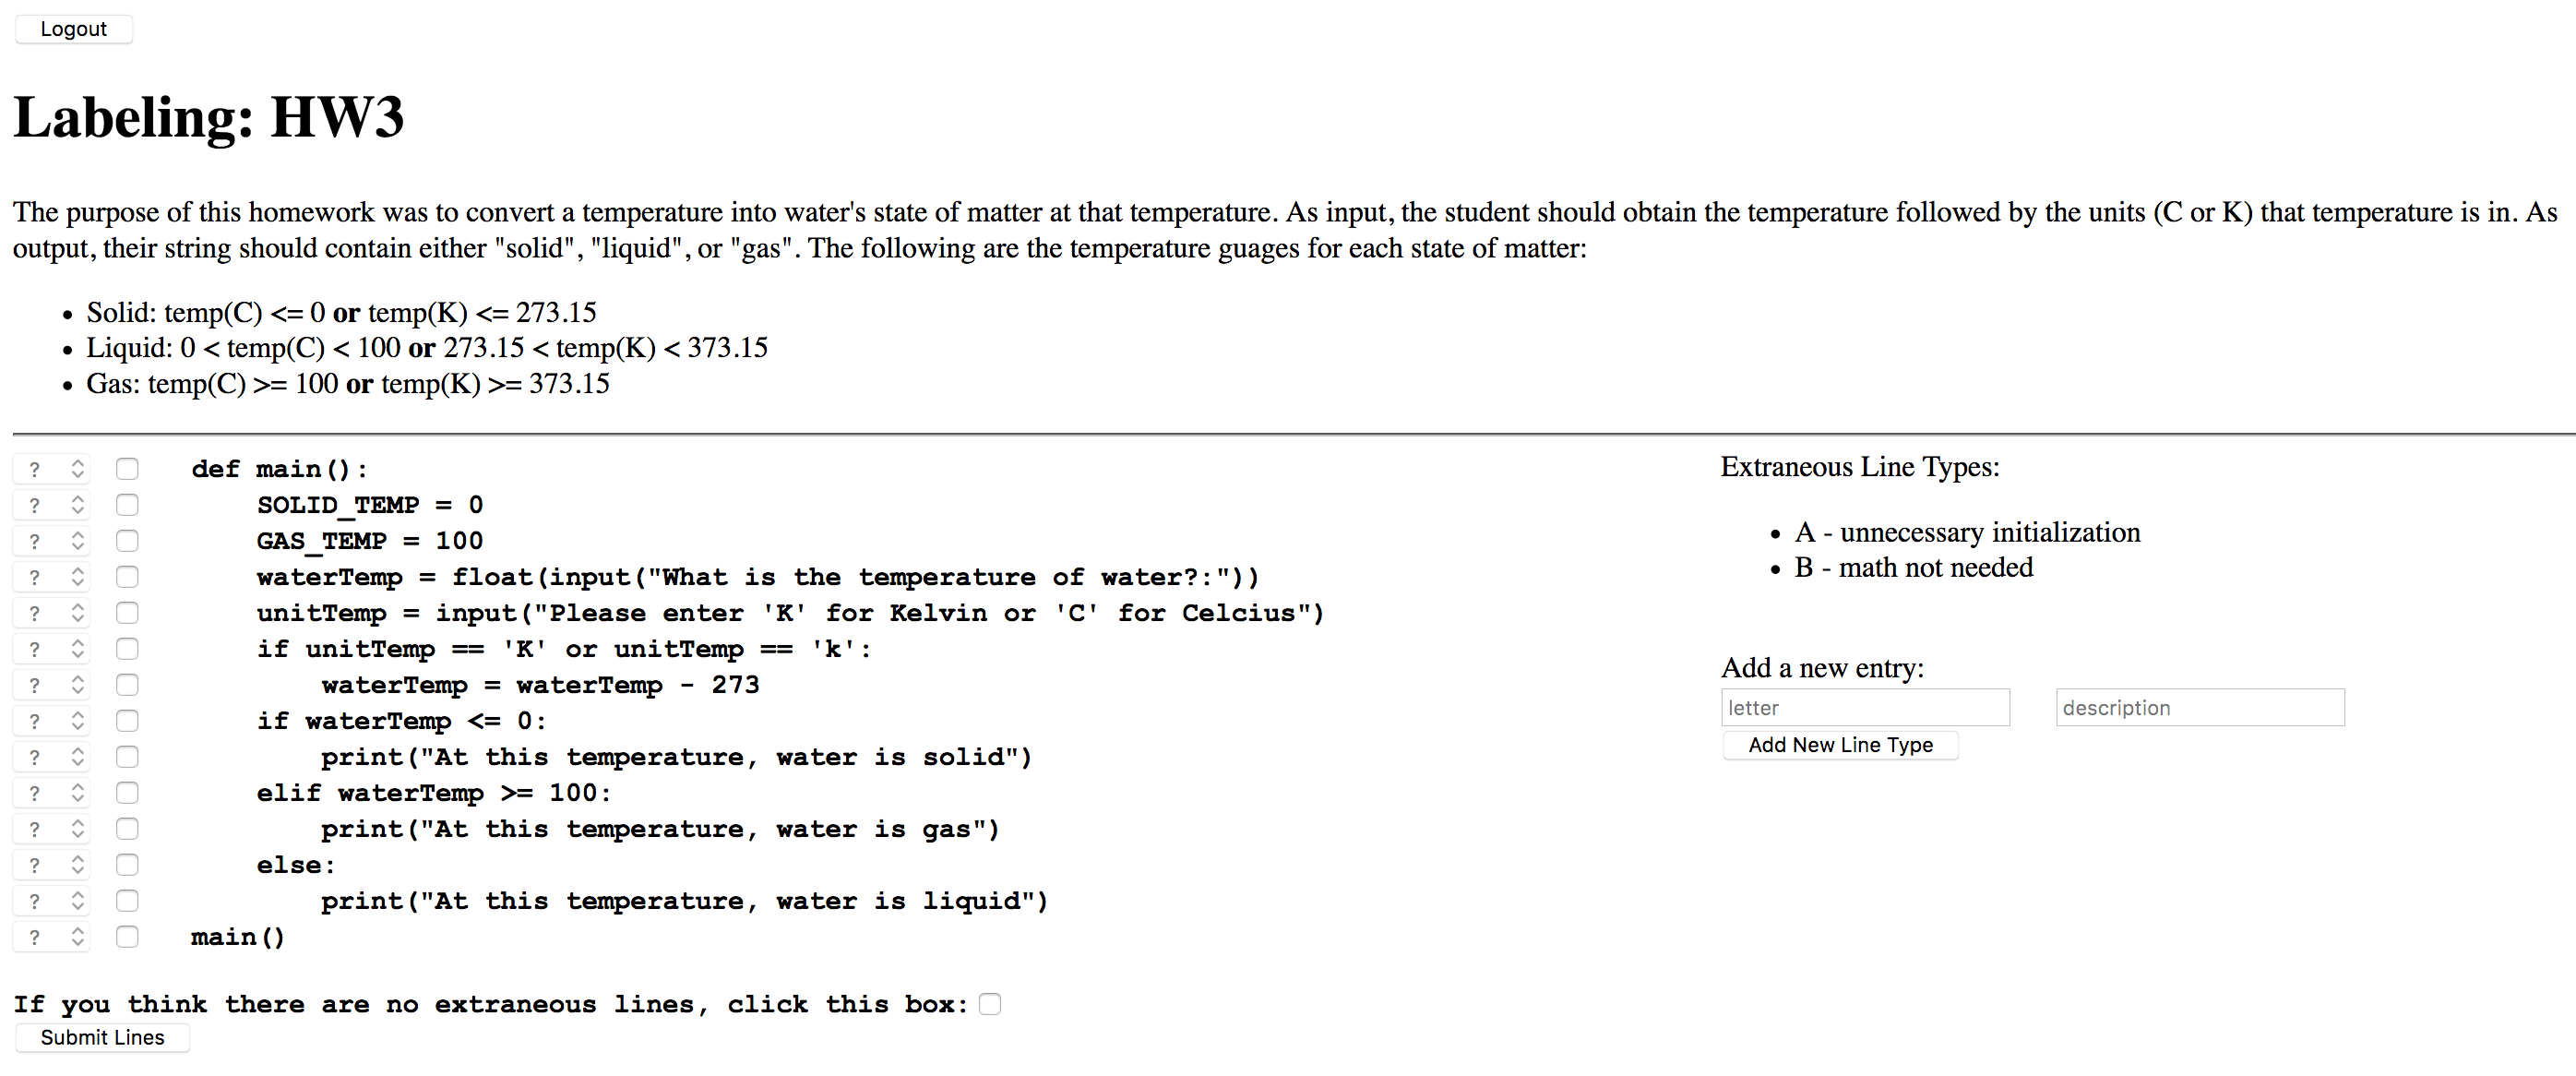
\includegraphics[width=\textwidth]{figures/webapp}
  \caption{Sample screen of a student labeling an assignment.}
  \label{fig:webapp}
\end{figure}

I built a custom web application to standardize the collection of labels. It allows me to easily collect different sets of labels from different people. Each user of the application reads every program, and determines which lines, if any, are extraneous. The application expedites the process of labeling, as flipping between assignments and keeping track of what has already been labeled is taken care of for the user. Figure \ref{fig:webapp} shows a sample screen for a single assignment. On the top of the page there is a description of the problem, including any guidelines as to what constitutes a correct solution, for their reference. On the left hand side of the screen they can view the source code line-by-line. A line is marked as extraneous by clicking a checkbox next to the line in this area, and choosing a letter from a drop-down menu. They were required to supply a short description of why they marked a line as extraneous. Each student developed a unique mapping of letter to description to save time in the labeling process. On the right hand side of the screen they can create a new mappings, and view any mappings they have already made. The short description helps me determine the reliability each student labeler. I can compare the lines that multiple students marked as extraneous, and use the descriptions the students provide to verify whether or not that label makes sense.

% Student A - Beatriz
% Student B - Harsh
% Student C - Keith
% Student D - Zoee

\subsection{Label Reliability}

The results of each experiment are heavily influenced by the reliability of the undergraduates who labeled the data sets. The labelers were carefully chosen such that their overall experience would better inform their selection of extraneous lines. To protect the identity of these students I will only refer to them as Student A, B, C, or D. Students A and D are female, while students B and D are male. Each student is undergraduate computer science major who has completed the gateway requirements, so they have all passed CMSC 201. Each student went on to be a teaching assistant for an introductory level course at UMBC (e.g. CMSC 201 - Introductory Programming in Python, CMSC 202 - Object Oriented Programming, or CMSC 341 - Data Structures). They have all helped many inexperienced students with homework assignments, and they were responsible for grading those assignments. Through the TA position, they have experience with identifying lines of code that are not necessary to satisfy the goal of a programming assignment. This is evident in the labels that were generated between the four students, as the descriptions match fairly well.

\vspace{2em}
\bottomcaption{Set of labels produced by Expert A.}\small
\begin{supertabular}{crrp{.5\textwidth}}
\label{labelsA}
Letter & Problem \#1 & Problem \#2 & Description \\ 
\toprule
A & 73 & 114 & unnecessary conversion of input to string \\
B & 1 & 3 & statement has no effect \\
C & 19 & 0 & conditional that has no effect \\
D & 1 & 0 & unnecessary print inside of input \\
E & 18 & 0 & statement never reached \\
F & 10 & 10 & unnecessary conversion of a variable type \\
G & 1 & 0 & unnecessary variable \\
H & 2 & 0 & while loop should've been if statement \\
I & 13 & 0 & duplicate code \\
Y & 0 & 202 & unnecessary start and/or step for range function \\
Z & 0 & 18 & loop that only executes once \\
\bottomrule
\textbf{Total:} & 138 & 347 & \\
\end{supertabular}
\vspace{2em}

Student A produced the set of labels described in \ref{labelsA}. The type of of line that was most identified by this student concerned an unnecessary start/stop with Python's range() function. This is a common mistake made by novice Python programmers as there are multiple default behaviors of this function. 

\vspace{2em}
\bottomcaption{Set of labels produced by Expert B.}\small
\begin{supertabular}{crrp{.6\textwidth}}
\label{labelsB}
Letter & Problem \#1 & Problem \#2 & Description \\ 
\toprule
A & 24 & 0 & Constant not used \\
B & 19 & 0 & Extraneous conditional where one or more conditionals have no affect in execution  \\
C & 117 & 122 & Extraneous type cast \\
D & 23 & 0 & Extraneous line duplication \\
E & 86 & 26 & Unnecessary line because it is extra information that does not achieve the program's core functionality requirement \\
F & 3 & 0 & Self Assignment \\
G & 453 & 44 & Extraneous syntax \\
H & 1 & 0 & Unnecessary return \\
I & 159 & 1 & No conditional required or should be default case (i.e. elif is not required if it is the base case)  \\
J & 1 & 0 & This line assumes that water is frozen if the temperature is less than K\_BOIL, which is not true. Water is frozen if below 273 \\
L & 3 & 20 & This operation should not be required \\
M & 6 & 18 & Unnecessary declaration  \\
N & 5 & 0 & Unnecessary operation exit() because using elif will ignore following cases if a previous if statement is true \\
O & 6 & 0 & This value is always overwritten in the following control flow, and is therefore always defined when it is actually used \\
P & 0 & 1 & Range defaults from 0 to n and the 0 is not required \\
Q & 0 & 13 & Unnecessary for loop \\
R & 0 & 2 & Counter not used \\
S & 0 & 11 & The default step of range is 1 \\
T & 0 & 108 & The default start of range is 0 \\
U & 0 & 4 & This function call / declaration does not accomplish anything \\

\bottomrule
\textbf{Total:} & 906 & 370 & \\
\end{supertabular}
\vspace{2em}

Student B produced the set of labels described in \ref{labelsB}.

\vspace{2em}
\bottomcaption{Set of labels created by Expert C}\small
\begin{supertabular}{crrp{.5\textwidth}}
\label{labelsC}
Letter & Problem \#1 & Problem \#2 & Description \\ 
\toprule
A & 71 & 37 & unnecessary print \\
B & 18 & 44 & unnecessary initialization \\
C & 66 & 0 & error-handling that does not contribute to solution \\
D & 18 & 6 & unnecessary conditional \\
E & 324 & 1 & an if/elif should be an elif/else \\
F & 71 & 111 & str() used on input() \\
G & 1 & 0 & unnecessary input \\
I & 6 & 0 & exit() not necessary \\

\bottomrule
\textbf{Total:} & 575 & 199 & \\
\end{supertabular}
\vspace{2em}

Student C produced the set of labels described in \ref{labelsC}. This is another sentence.

\vspace{2em}
\bottomcaption{Set of labels created by Expert D}\small
\begin{supertabular}{crrp{.5\textwidth}}
\label{labelsD}
Letter & Problem \#1 & Problem \#2 & Description \\ 
\toprule
A & 2 & 0 & opportunity for compound assignment \\
B & 116 & 124 & unnecessary casting \\
C & 13 & 0 & semicolon to end line \\
D & 2 & 0 & unnecessary return \\
E & 2 & 0 & self assignment \\
F & 560 & 208 & unnecessary parenthesis \\
G & 17 & 6 & added to assignment \\
H & 4 & 0 & Debug statement \\
I & 1 & 0 & condition always true or always false \\
J & 2 & 7 & unused variable \\
K & 2 & 5 & renamed variable \\
L & 1 & 0 & print in input \\
M & 0 & 6 & Always loops once \\
N & 0 & 3 & performs no function \\
O & 0 & 7 & unnecessary initialization \\
P & 0 & 4 & unnecessary parameters \\

\bottomrule
\textbf{Total:} & 722 & 370 & \\
\end{supertabular}
\vspace{2em}


Student D produced the set of labels described in \ref{labelsD}.

Each of the four students identified some form of unnecessary casting of variable type.


\textcolor{blue}{
\begin{itemize}
    \itemsep-1.5em 
    \item [\textbf{TODO:}]
    \item Talk about what each student did individually
    \item Talk about how the labels relate to each other.
    \item Support the conclusion that the generated labels are reliable 
    \item Show the label counts visually, do not just write numbers in prose
\end{itemize}}

\subsection{Problem 1}
CMSC 201 received 466 unique submissions for this problem in Fall 2016. Table [\textbf{reference}] shows the breakdown of how those lines were labeled by the students. 

\subsection{Problem 2}
CMSC 201 received 467 submissions for this problem during Fall 2016. Table [\textbf{reference}] shows the breakdown of how those lines were labeled by the students.
\textcolor{blue}{
\begin{itemize}
    \itemsep-1.5em 
    \item [\textbf{TODO:}] Something similar to the following among everyone
\end{itemize}}
Although Student A identified almost twice as many unique files for this problem, the average number of lines per file is roughly the same. The culprit seems to be that Student A considers an unnecessary start and/or step in the range() function to be extraneous, as that account for more than half of the lines they identified as extraneous.

\section{Experiments}
Two experiments were carried out with my method using the labeled data provided by the undergraduate students. My method was run seven different different times, once for each combination of the three different types of dependencies. Each of these runs are compared to each set of labeled data, as well as the intersection of the data sets. Different runs help to visualize the impact that different dependency types have on detecting extraneous lines of code. I compute the accuracy, the sensitivity, and the specificity of each run.


%I will likely only compare the results of my experiments to the lines of code that were identified as extraneous by all four students. the question is: is that ok to do?

\subsection{Problem 1}

% each of the following items in this list are one experimentation method that I will include. I need to rerun a few of these results, and figure out some numbers before I write this up. Do I need to include all 7 permutations in my analysis, or should I justify not showing all of them somehow? Also, I need to figure out a better way of graphically representing the information 

\subsubsection{Analysis}
This is where I talk about specific intuitions regarding the first problem.

\subsection{Problem 2}
This is where I describe the setup for the second problem.

\subsubsection{Analysis}
This is where I talk about specific intuitions regarding the second problem.

\section{Conclusion}
This is where I wrap up my contribution(s) to science.

